\chapter{Dados}

\section{Dados Utilizados \label{se:dados_crus}}

Os dados em estudo são do mercado energético espanol, retirados do site :
https://www.esios.ree.es/es


\csvautotabular{../data/indicators_metadata.csv}


\subsection{Aquisição dos Dados (depth 2)}

No ambito da automatização destes dados foi modificado o repositorio ESIOS (ref) para ser usado como uma biblioteca de python, aberta, em pypi.
Sendo uma ferramenta mais facilmente acessivel para a extrair dados do mercado espanhol:
https://pypi.org/project/pyesios/



\section{Estudo dos dados  \label{se:dados_estudo}}

Os dados que propunho a prever são: "UpwardUsedSecondaryReserveEnergy", "DownwardUsedSecondaryReserveEnergy"

\begin{figure}[H]
  \centering
  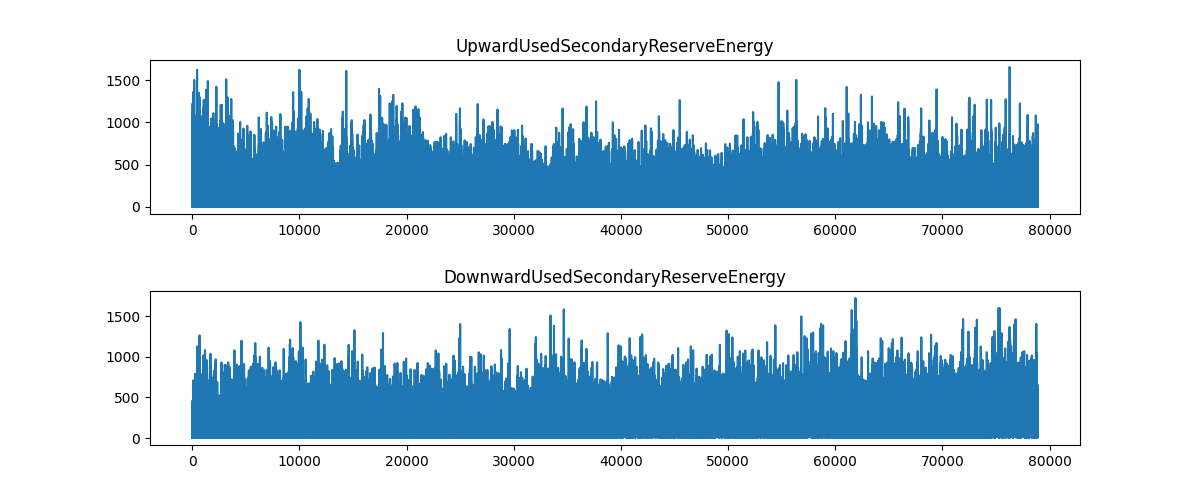
\includegraphics[width=0.8\textwidth]{../plots/targets_timeseries.png}
  \caption{Serie Temporal dos dados alvo}
  \label{fig:target_timeseries}
\end{figure}

Para termos uma melhor percepção dos mesmos segue algumas janelas temporais mais pequenas.

\begin{figure}[H]
  \centering
  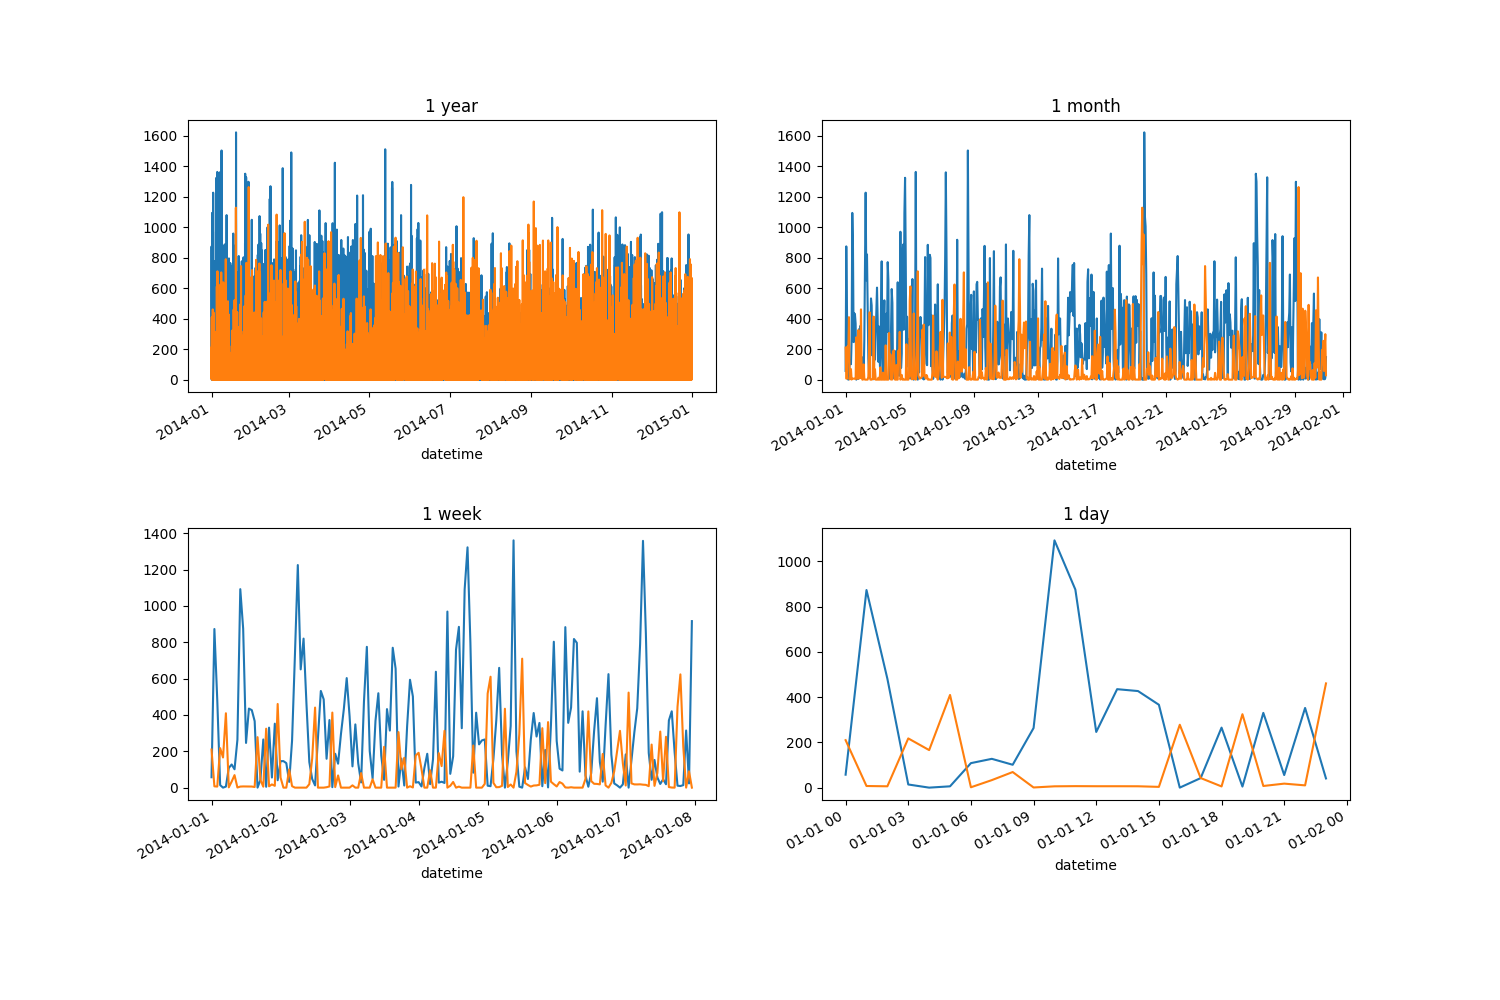
\includegraphics[width=0.8\textwidth]{../plots/target_timeseries_windows.png}
  \caption{Janelas Temporais dos dados alvo}
  \label{fig:target_timeseries_windows}
\end{figure}


Estas mostram claramente que ambos os atributos mantêm um comportamento tanto discreto, como linear, isto é, que ou existe algum valor, ou é zero, e se existe valor este tem comportamento linear.



A distribuição destes dados é claremente exponencial. O que é importante para a escolha de alguns parametros no modelação

		
\begin{figure}[H]
  \centering
  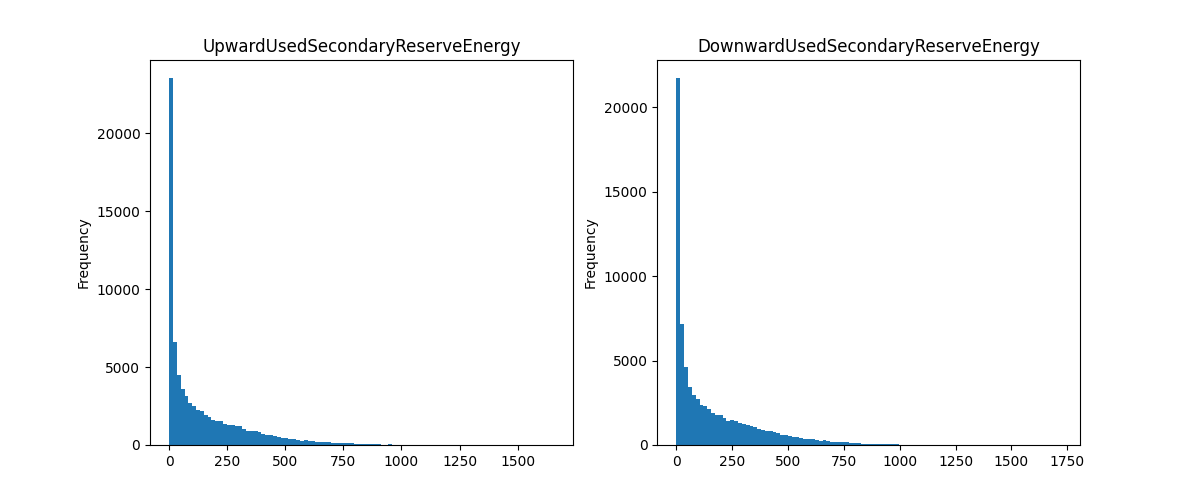
\includegraphics[width=\textwidth]{../plots/target_histograms.png}
  \caption{Frequência dos dados alvos}
\end{figure}


\subsection{Correlações}

\subsubsection{Correlações entre atributos}

Os modelos vão depender bastante de correlação entre variaveis.
Nesta secção queremos tentar identificar se há visiveis relações entre as variaveis, e se há relações temporais  visiveis nas colunas alvo.



\begin{figure}[H]
  \centering
  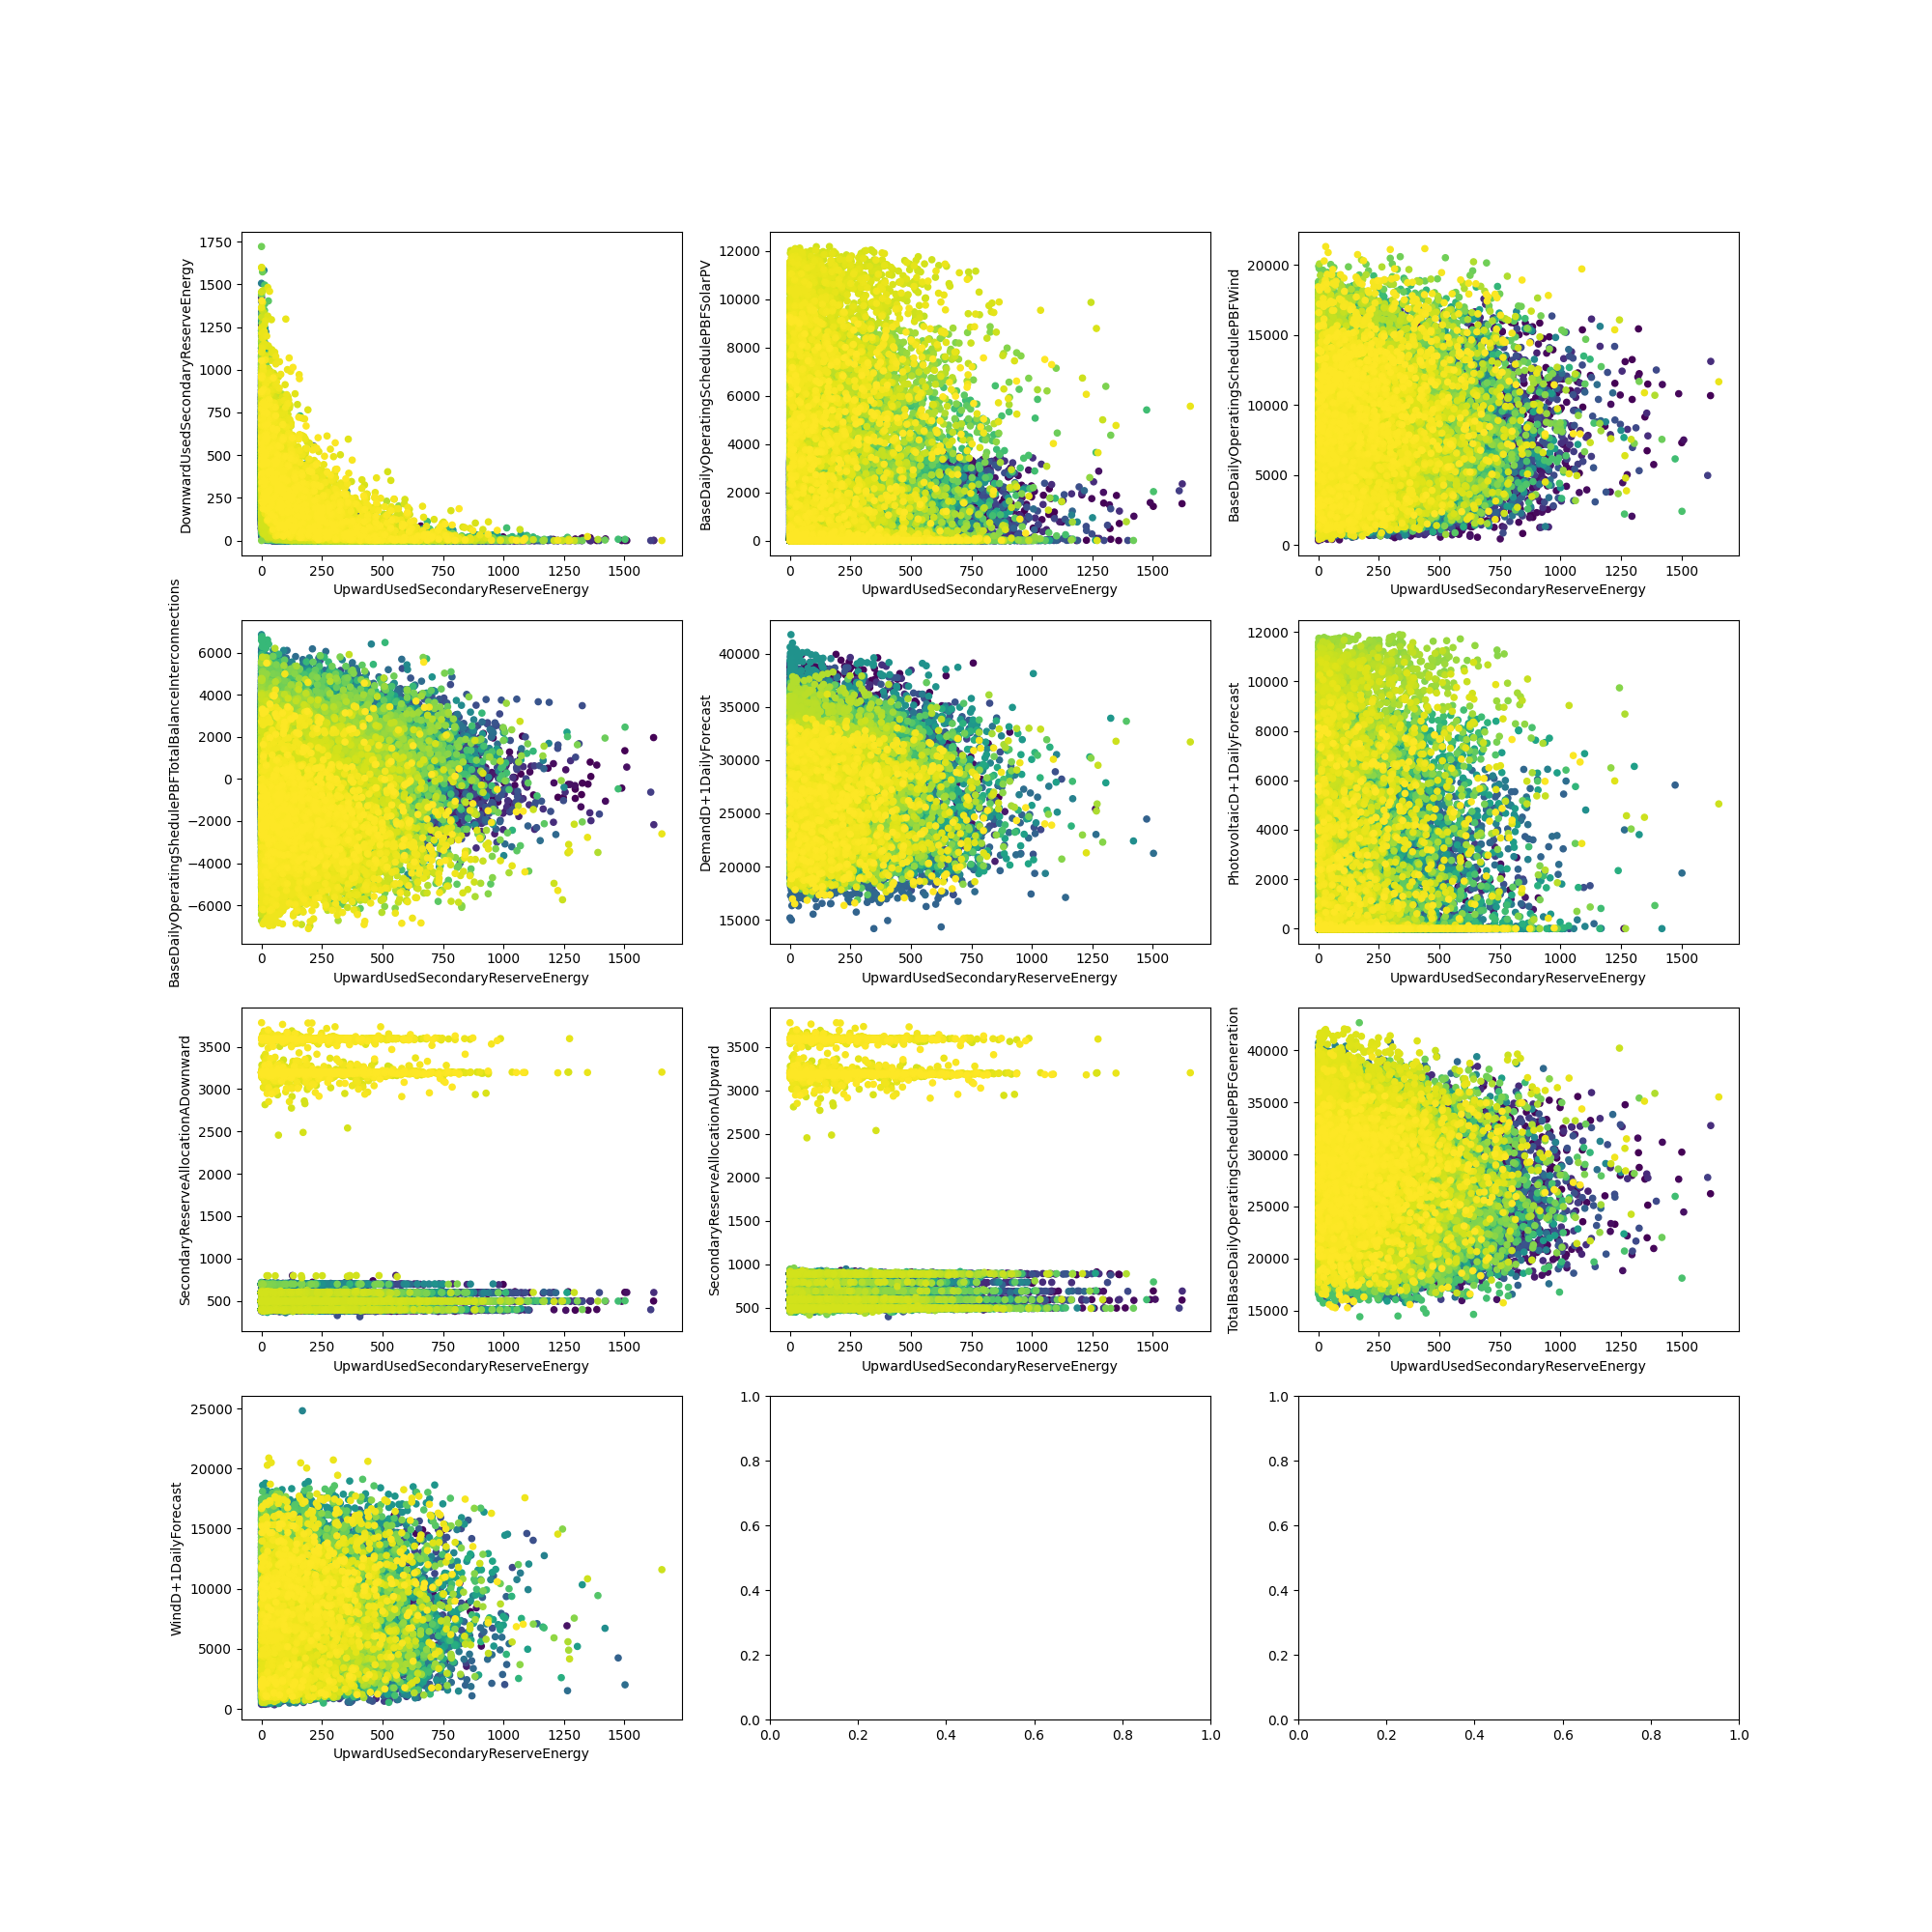
\includegraphics[width=\textwidth]{../plots/feature_correlation.png}
  \caption{Correlação entre atributos}
\end{figure}

As correlações entre variveis parecem muitos escassas o que apresenta já que a previção deste dados usando estas variaveis vai ser um problema dificil.
Por norma é feito uma seleção de  atributos baseado nestas correlações, eliminando assim os atributos que ajudam menos, ou ate prejudicam os modelos.
Segue os valores de correlação onde podemos ver numericamente que existe muito pouca correlação entre os atributos.

\begin{figure}[H]
  \centering
  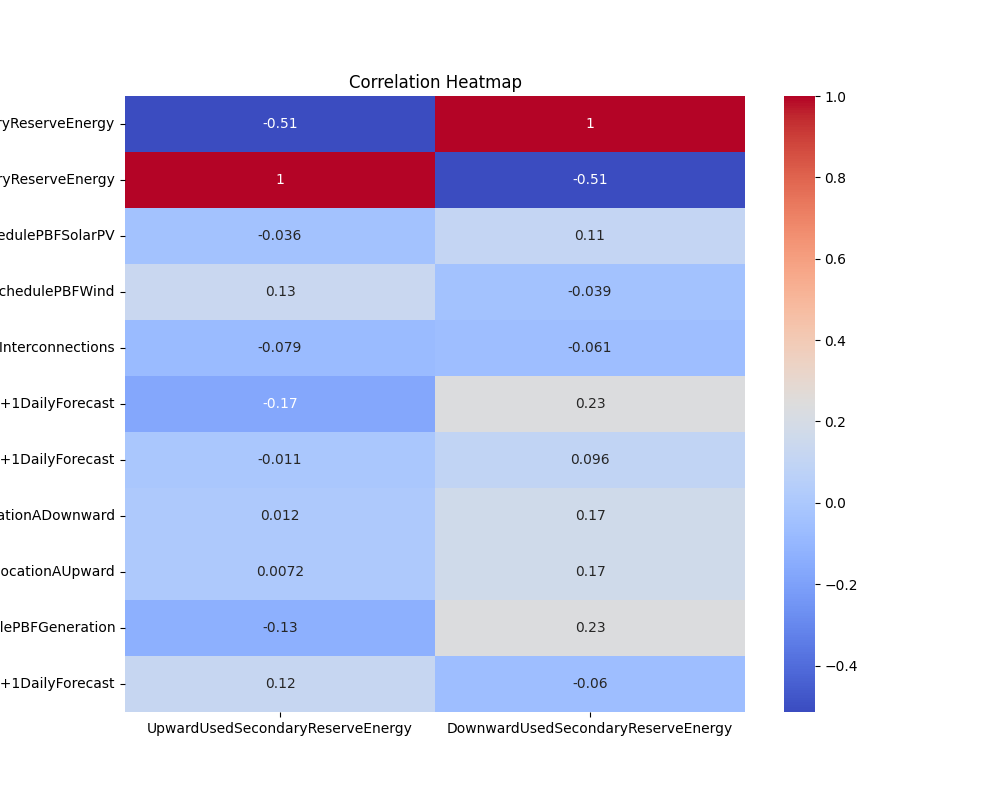
\includegraphics[width=\textwidth]{../plots/correlation_heatmap.png}
  \caption{Valores de correlação entre atributos}
\end{figure}

\subsubsection{Correlações Temporais}

\begin{figure}[H]
  \centering
  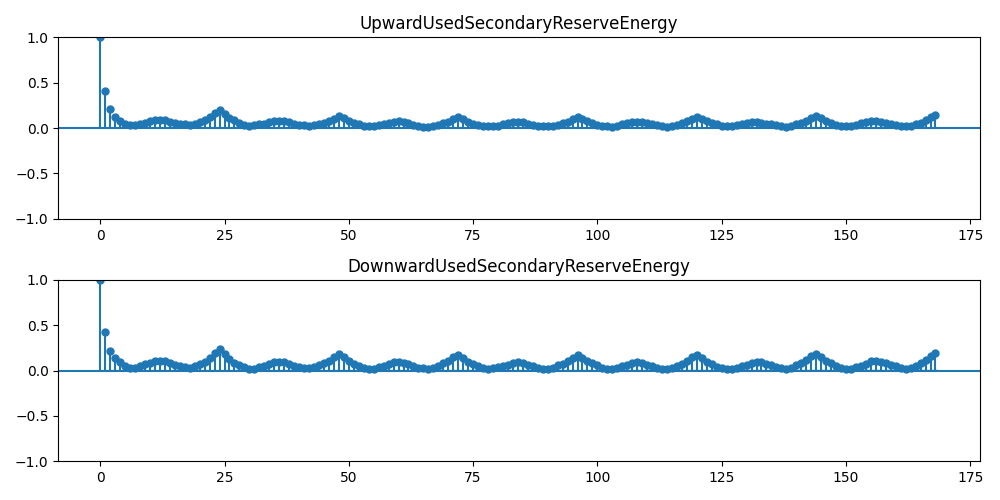
\includegraphics[width=\textwidth]{../plots/autocorrelation.png}
  \caption{Serie Temporal dos dados alvo}
\end{figure}


A autocorrelação, em ambos os "targets", é mais forte nas 3 horas mais proximas, e nos pontos com diferença de 12 e 24 horas.
É de notar que estes valores são baixos, prometendo já tambem uma baixa regressividade temporal.
Outro ponto a denotar é que os objectos não têm um comportamento completamente linear, i.e., parece existir um comportamento discreto na questão ser alocado ou não esta reservas secundárias, e caso seja alocado, aí existir alguma linearidade.
Logo qualquer tipo de modelação terá de resolver primeiramente este problema.

Estas relações mostram que em termos de atributos usados vai ser um desafio complicado para qualquer tipo de modelo.

No âmbito desta disserteção queremos verificar a qualidade das previsões usando estes mesmo atributos, logo, não será feita seleção dos mesmos.

A nível da relação temporal, a maior parte dos modelos que iremos testar aplica um janela na dimensão temporal, usando todos os valores nessa janela, e aplicando os pesos nessas distancias que mais se enquadram. Logo também não é relevante escolher apenas as distancias temporais com maior correlação, pois os modelos vão fazer essa pesagem.

\subsection{Agrupamento \label{se:clustering}}

Uma das possibilidades na modelção será a utilização de grupo de valores, classes, em conjunto com a linearidade.
Devido ao comportamente não exclusivamente linear (tenho de procurar um nome para isto) é tambem estudado as possiveis agregassões (clustering) em que podemos dividir os valores em classe.
Tendo por base que uma das classes é o valor zero, devido ao comportamento não linear desta série, vamos apenas testas quantos, e quais, as melhores classes em que podemos dividir os dados.
É realizado o teste de silhoeta (ref) e o teste do cotovelo (ref), que se baseiam nos resultados de silhoeta do modelo GMM (ref) e nos valores de inercia do modelo K-Means (ref). 

\begin{figure}[H]
  \centering
  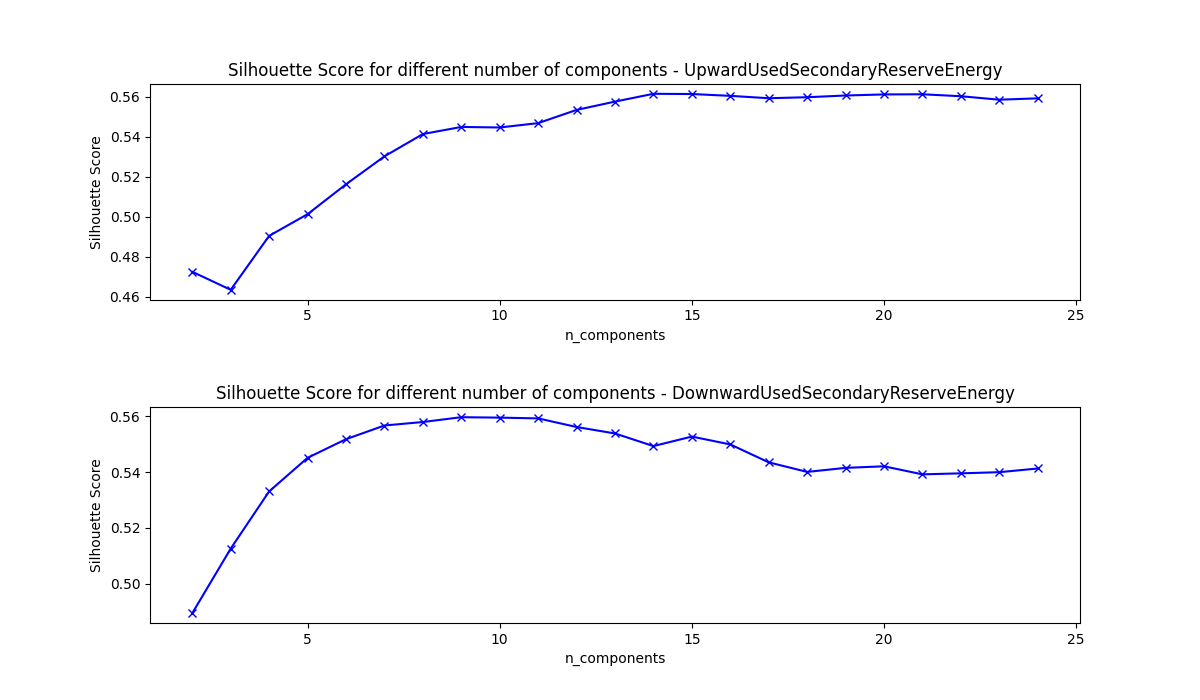
\includegraphics[width=\textwidth]{../plots/silhouette_score.png}
  \caption{Serie Temporal dos dados alvo}
\end{figure}


\begin{figure}[H]
  \centering
  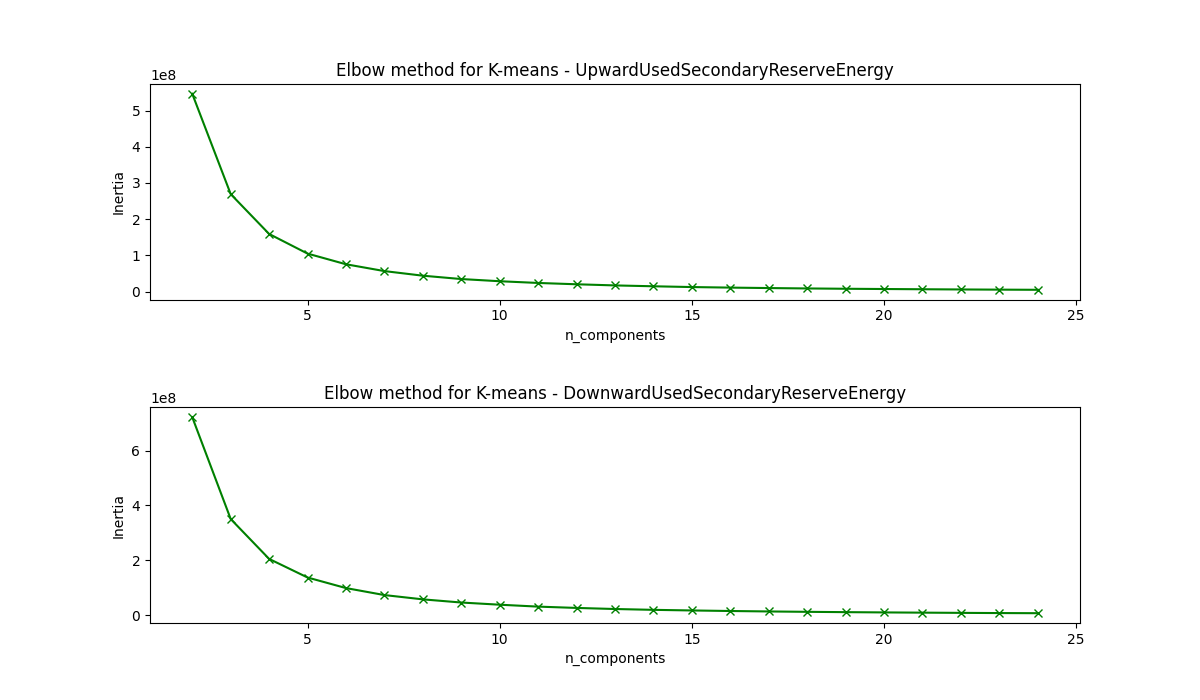
\includegraphics[width=\textwidth]{../plots/elbow_test.png}
  \caption{Serie Temporal dos dados alvo}
\end{figure}


Ambos os casos apontam um assintota na relação interna dos clusters, a partir de cerca de 5 clusters, sendo que o melhor valor dos verificados seria com 14 clusters em "UpwardUsedSecondaryReserveEnergy" e 9 em "DownwardUsedSecondaryReserveEnergy".
Para a nossa questão, queremos algumas classes, mas quanto menos classes mais facil será para os modelos correctammente identificar a que classe pertence. Logo para os valores apresentados, escolhemos 5 clusters, sendo que este já pode ser um numero elevado de classes, logo usemos 3 clusters se os modelos tiverem muuita dificuldade com 5.
O método do cotovelo apresenta como numero ideal de clusters 4, mas sendo que K-Means é um metodo mais apropriado para distribuições normais, em que a distancia nos limites dos clusters não varia, deixamos apenas informativo.

O histograma das divisões pode ser visto em baixo. O valor é a sua própria classe para além das apresentadas.

\begin{figure}[H]
  \centering
  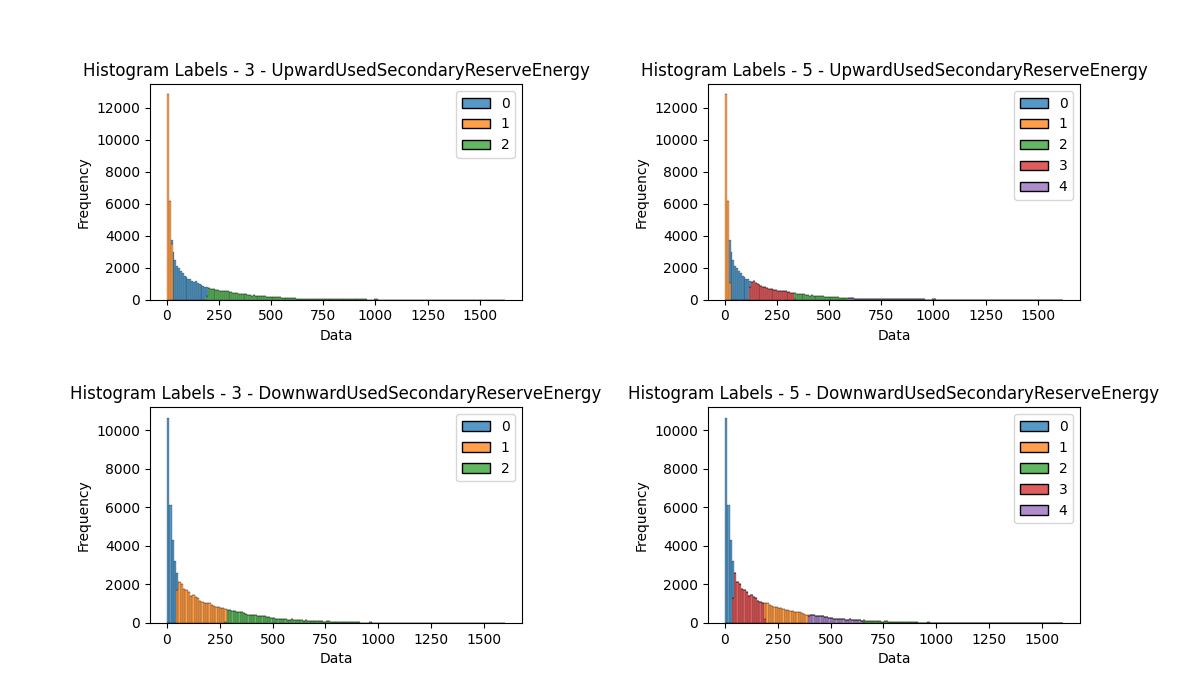
\includegraphics[width=\textwidth]{../plots/clusters_histogram.png}
  \caption{Histograma das classes}
\end{figure}

Os limites retirados são:

\csvautotabular{../data/cluster_limits.csv}



\section{Tratamento dos dados  \label{se:data_treatment}}

Normalizaçao
A normalizaçao foi deixada por ser aprendida nos modelos, sendo que todos têm como segunda camada, uma de normalização.

Limpeza

Podemos ver pelos graficos seguintes que a existem alguns outliers, sendo estes definidos como 3 desvios padrão de distância à média.

graphhhhhhhhh


No caso de "" e "" existe um grande salto nos valores logo o aqui os dados são partidos e estudados os outliers nas duas diferentes zonas.
A limpeza destes dados é feita apenas substituindo pelo ................................................

Fica também como motivo de estudo se a remoção deste outliers ajuda na modelação.


Estudemos tambem o caso de dados em falta. Alguns destes atributos têm certas entras vazias, e como podemos ver alguns não têm alguns anos inteiros.
Como queremos usar o maximo de dados possiveis iremos usar tecnicas de imputing nesses dados 
............................................
imputing
https://arxiv.org/abs/2102.03340

cleaning
	outliers
		naquela parte que parte fazer a limpeza em duas vezes
		melhora se tirarmos os outliers?
		
	imputing de missing data
	
features adicionais:
	apenas as temporais	

Por ultimo foi adicionado ao dados mais atributos, sendo eles todos de cariz temporal. É adicionado atributos correspondentes à hora, ao dia do ano, ao dia da semana, ao dia do mês, mês, ano. TODO


\section{Considerações adicionais  \label{se:dados_plus}}

Talvez aqui uma secçao para finalizar e mostrar algumas coisas
